\section{Chapter 8. Basic Concepts of Chemical Bonding}

\secttoc

{\footnotesize
\begin{multicols}{3}
\begin{compactenum}
    \item Lewis symbols for atoms and ions
    \item Lattice energy. Rank based on ion sizes and charges.
    \item $e^-$ config and octet rule to draw Lewis structure
    \item Electronegativity differences and non-polar/polar covalent and ionic
        bonds
    \item Charge separation in diatomic molecules based on dipole moment
        and bond length
    \item Formal charges, ID dominant Lewis structures
    \item Recognize molecules where resonance structures are needed, draw
        dominant res. struct.
    \item All exceptions to octet rule
    \item Relationship between bond type (single, double, triple),
        bond strength/enthalpy, and bond length
    \item Bond enthalpies to estimate enthalpy changes for gas-phase reactants
        and products
\end{compactenum}
\end{multicols}
}

\begin{mdframed}
\subsection{Lewis Structures}
\begin{multicols}{2}
\begin{compactdesc}
\item[Representation] of electron arrangement and bonds. Valence $e^-$ are
    drawn as dots around atom, shared pairs are lines between atoms.
    Most atoms require 8 valence $e^-$, H needs 2.
\item[Electron Config of Ions] remove or add $e^-$ to highest n, then l.
\item[Formal Charge] valence - $\frac{1}{2}$bonding - non-bonding
\item[Most common Lewis structure] has the lowest formal charge
\item[Not enough valence] electrons could cause a multiple bond.
\end{compactdesc}

\subsection{Resonance structures}
The actual bonds of a substance with multiple valid bonding schemes cannot be
modeled using a single Lewis structure. Examples, Benzene and \ce{O3}:
\begin{figure}[H]
    \centering
    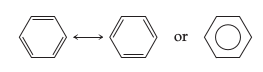
\includegraphics[width=0.24\textwidth]{benzene.png}
    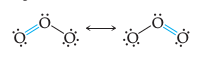
\includegraphics[width=0.24\textwidth]{ozone.png}
\end{figure}


Benzene's arrangement confers special stability to molecules.

\subsection{Exceptions to the Octet Rule}
\begin{compactdesc}
\item[Odd number of $e^-$] \ce{BF3} has resonance and six valence around Boron,
    \ce{NO} has 11 valence electrons
\item[Hypervalent] molecule or ion has more than an octet around central atom
    Only period 3++, due to larger size.
\item[Octet gives unfavorable] distribution.
\item[Large atom] surrounded by large number of small electronegative atoms,
    enough to overpower the octet rule.
\item[Electron configuration] shows distribution of $e^-$ in orbitals.
    $\ce{F}: [\ce{He}] 2s^2 2p^5$
\end{compactdesc}

\begin{figure}[H]
    \centering
    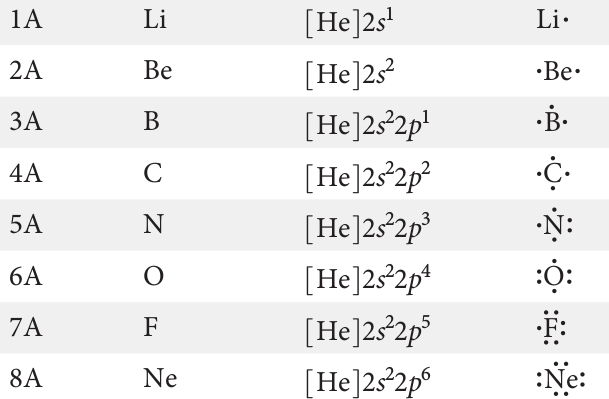
\includegraphics[width=0.3\textwidth]{lewis_basics.png}
\end{figure}

\end{multicols}
\end{mdframed}



\begin{mdframed}
\begin{multicols}{2}
\subsection{Ionic Bonds}
\begin{compactdesc}
\item[Lattice energy] indicates energy needed to separate an ionic substance
    into its gaseous components: \ce{AB -> A+ (g) + B^- (g)}
\item[Related] to Coulomb's law for particles.
\item[Born-Haber cycle]
    Used to calculate the elusive lattice energy using several known energies
    and Hess's law.
\end{compactdesc}




\subsection{Strengths and Lengths of Covalent Bonds}
\begin{compactdesc}
\item[Strength] is determined by energy needed to break the bond
\item[Bond enthalpy] $\Delta H$ needed to break a bond in one mole of a gaseous
    substance: \ce{Cl2(g) -> 2Cl(g)}. Represented as D(\ce{Cl-Cl})
\item[Enthalpies of Reactions] can be determined using bond enthalpies, even
    if $\Delta H_f^\circ$ are not known for all involved.
    Imagine two steps: energy to break all bonds as needed, energy to form new
    bonds.
\item[Bond length] decreases with increasing number of bonds between two atoms.
\item[Smaller bond length] larger $\Delta H$
\end{compactdesc}

\begin{figure}[H]
    \centering
    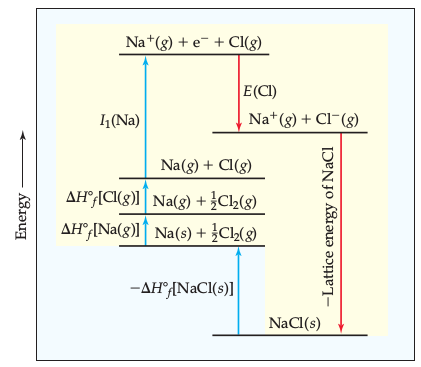
\includegraphics[width=0.4\textwidth]{Born_Haber_cycle.png}
\end{figure}

\end{multicols}
\end{mdframed}


\begin{mdframed}
\subsection{Bond Polarity and Electronegativity}
\begin{multicols}{2}
\begin{compactdesc}
\item[Electronegativity] ability of an atom in a molecule to attract $e^-$.
    Based on ionization energy, electron afinity and other properties.
    \textbf{Trend:} increases to the top-right
\item[Bond polarity] equality of $e^-$ distribution in covalent bond
\item[Nonpolar covalent] equal electron sharing. Difference in
    e.neg = 0.
\item[Polar covalent] not equal electron sharing. Partial charge represented
    as $\delta +$ and $\delta -$. In HF, H has partial positive, in \ce{H2O}
    H has partial negative. Difference in e.neg about 0.5.
\item[Ionic bonds] very unequal electron sharing. Difference in e.neg $\gg 0.5$.
\item[Dipole moment] indicates direction and magnitude of partial charge.
    Relates to charge and radius: $\mu = Q \cdot r$.
\end{compactdesc}

\begin{figure}[H]
    \centering
    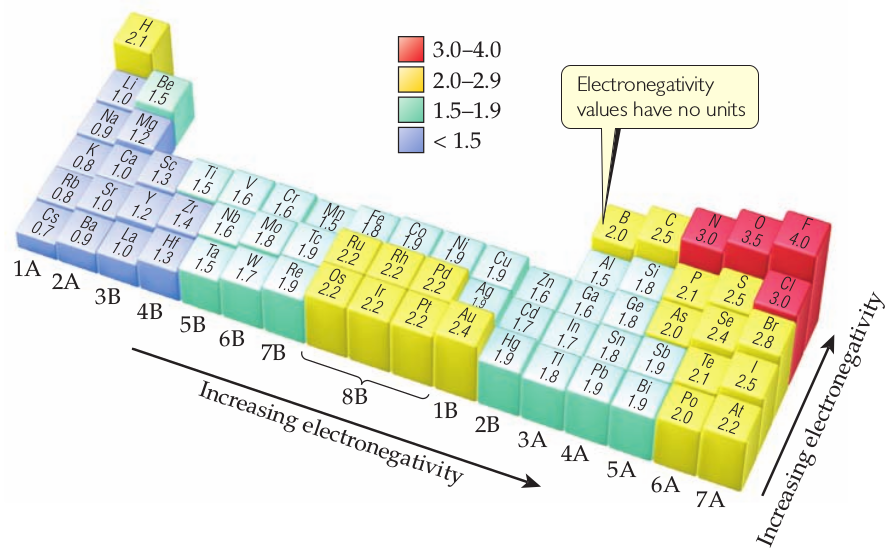
\includegraphics[width=0.5\textwidth]{electronegativity_table.png}
\end{figure}
\end{multicols}
\end{mdframed}

